\section*{Abstract}
We present preliminary studies into the development of efficient and effective strategies for the usage of LSST in optical follow-up of gravitational wave events. Specifically, we focus on the detection and characterization of kilonovae across a wide range of ejecta properties and composition. We show that the main LSST survey will achieve an average efficiency for kilonova detection of \apx3\%, with only a handful of sources characterized well enough for detailed study. In contrast, triggered target-of-opportunity follow up with a minimal time investment of a few hours per night will be able to detect a wider range of kilonova models, provided observations commence promptly after the GW trigger. This suggests that LSST has the opportunity to play an important role in the growth of multi-messenger astronomy by facilitating highly efficient kilonova searches.

\clearpage
\section{Introduction}
\label{sec:ch6_intro}
The discovery of an optical counterpart associated with the the binary neutron star merger GW170817 was a watershed moment in the development of joint gravitational wave and electromagnetic (GW-EM) astronomy \citep{LIGOGW170817,LIGOMMAPaper,Arcavi+17,Coulter+17,GW170817DECam,Valenti+17}. Subsequent modeling of the optical light curves revealed behavior consistent with that of a kilonova \citep{Cowp+17,Kilpatrick+17,Tanaka+17,Villar+17b, Tanaka+18}, an optical/NIR transient expected to accompany compact object mergers involving at least one neutron star \citep[see e.g.,][]{Metzger2017}. The discovery of this optical transient has opened up numerous new and exciting science possibilities. These include studies into the host galaxy \citep[NGC4993, see e.g.,][]{Blanchard+17,Cantiello+18}, constraining the neutron star equation of state \citep[see e.g.,][]{Radice+18}, and even making independent measurements of the local Hubble Constant \citep[H$_0$, see e.g.,][]{LIGOH0,Guidorzi+17}.

If we wish to build upon the success of GW170817 and push into new realms of joint GW-EM science then we must work to facilitate future detections of both gravitational wave sources {\em and} their associated electromagnetic counterparts. A key component of future searches for gravitational wave events is improving the ability of the interferometer network to localize sources on the sky. Over the next several years, as both Advanced LIGO and Virgo reach their design sensitivity, it is expected that they will be able to localize compact binary mergers to sky areas of approximately tens to hundreds of deg$^2$ \citep{LIGOLocalization,ChenHolz16}. Major improvements to sky localization will continue over the next decade as two additional interferometers, KAGRA in Japan \citep{KAGRA} and LIGO-India \citep{LIGOIndia}, join the network. In this five detector regime, compact binary mergers will be localized to just $\apx10$~deg$^2$ \citep{Fairhurst2014,ChenHolz16}.

Similarly, improving our ability to identify electromagnetic counterparts in these localizations will rely on using the next generation of optical facilities that are soon to be coming online. One such facility, the Large Synoptic Survey Telescope \citep[LSST,][]{Ivezic+09}, will be the premiere time-domain instrument in the Southern hemisphere during the next decade. LSST boasts an 8.4-m primary mirror and a 9.6 deg$^2$ field-of-view. This powerful combination of large aperture and wide field-of-view makes LSST uniquely suited to the task of gravitational wave follow-up. The field-of-view is particularly well matched to the expected localization regions allowing LSST to observe a high fraction of the localization probability in just one or two pointings.

Of particular importance is the development of efficient and effective strategies for gravitational wave follow-up with LSST. This first involves understanding both the rate and properties of kilonovae detected in the LSST main survey. This was investigated by \citet{Scolnic+18} who injected model light curves of the kilonova associated with GW170817 \citep[hereafer just ``GW170817" for simplicity][]{Cowp+17} into the LSST cadence. They found that LSST should detect $\apx7$ GW170817-like kilonovae per year during the ten year main survey. However, these kilonovae were observed only a few times per event, leading to poorly-sampled light curves. As a result, real-time identification and modeling of these kilonovae will be difficult. Furthermore, these kilonovae are detected far beyond the sensitivity horizon for LIGO, meaning that an association between these kilonovae and a gravitational wave detection is unlikely. This suggests that triggered target-of-opportunities may be a more promising approach.

Here we expand on the groundwork established by \citet{Scolnic+18} along two new avenues. First, we expand the range of kilonovae models considered in the LSST main survey. This is accomplished by considering a wider range of ejecta masses and composition to fully explore the potential range of kilonovae brightness and timescales. Second, we expand beyond the main survey cadence to discuss the benefits of targeted target-of-opportunity (ToO) observations when compared to the main survey.

This work is organized as follows: In \cref{sec:ch6_models} we describe the expanded range of kilonovae models used in our simulated observations. In \cref{sec:ch6_obs} we describe our methodology for simulating LSST observations using both OpSim for the main survey cadence and SNANA for target-of-opportunity observations. In \cref{sec:ch6_analysis} we present the results of our simulated observations. Lastly, discussions and conclusions are presented in \cref{sec:ch6_conc}.

All magnitudes presented in this work are given in the AB system unless otherwise noted. Cosmological calculations are performed using the cosmological parameters $H_0 = 67.7$ km s$^{-1}$ Mpc$^{-1}$, $\Omega_M = 0.307$, and $\Omega_{\Lambda} = 0.691$ \citep{Planck2016}.

\clearpage
\section{Kilonova Models}
\label{sec:ch6_models}
A kilonova is an isotropic optical/NIR thermal transient produced by the merger of a compact object binary containing at least one neutron star such as a binary neutron star (BNS) or neutron star-black hole binary (NS-BH). In either scenario, the merger produces a small amount of ejecta ($\Mej \lesssim 0.1 \msun$), which is typically neutron-rich. As the ejecta expands from nuclear densities, it will synthesize heavy elements via $r$-process nucleosynthesis. These heavy nuclei are unstable and will decay back to stability depositing energy into the ejecta which powers the kilonova emission \citep{LP98,Metzger+10,BarnesKasen13,TanakaHotokezaka13,Metzger2017}.

The exact nature of this kilonova emission depends strongly on the composition of the ejecta, specifically the neutron-richness which is parametrized by the electron fraction ($Y_e$). If the material is very neutron-rich ($Y_e \lesssim 0.3$), then the ejecta will undergo strong $r$-process nucleosynthesis, producing very heavy elements ($A > 140$), particularly those in the lanthanide and actinide series. As a result of these heavy elements, the ejecta will have a high opacity $(\kappa \gtrsim 10 \cspg)$. The resulting ``red" kilonova will then be faint with a peak bolometric luminosity of $L_p \apx10^{40}-10^{41} \ergs$, red ($i-z \gtrsim 0$), and exhibit a timescale of $t_p \apx1$ week \citep{BarnesKasen13,TanakaHotokezaka13}. If instead the material is less neutron-rich ($Y_e \gtrsim 0.3$), then the ejecta will undergo light $r$-process nucleosynthesis, producing Fe-group and light $r$-process elements ($A \lesssim 140$), and the ejecta will have a lower opacity $(\kappa \apx0.1 \cspg)$. The resulting ``blue" kilonova will be brighter $L_p \apx10^{41}-10^{42} \ergs$, bluer ($i-z \lesssim 0$), and exhibit a shorter timescale of $t_p \apx1$ day \citep{Metzger+10,MetzgerFernandez14}.

In practice, the observed kilonova will exhibit some combination of both ``red" and ``blue" features. This behavior was seen in the kilonova associated with GW170817, where the multi-band optical/NIR light curve was best described by a three-component model consisting of ``red"  $(\kappa \apx10 \cspg)$, ``purple"  $(\kappa \apx3 \cspg)$, and "blue"  $(\kappa \apx0.1 \cspg)$ $r$-process powered components. This three-component approach was first suggested by \citet{Tanaka+17} as a good approximation to the more complex opacity behavior seen in detailed radiative transport simulations. The three-component approach is also physically motivated as the different emission components may arise from different sources of ejecta present in the merger. The ``blue`` emission may arise from neutron-poor ejecta in the polar region where material is shock-heated during the NS collision \citep{Oechslin+07,Bauswein+13a,Sekiguchi+16} or if the ejecta is irradiated by neutrinos from a long-lived merger remnant \citep{FernandezMetzger13,Just+15,Kasen+15}. The ``purple" and ``red" emission may arise from ejecta produced in the tidal tails during merger \cite{Rosswog+99,Hotokezaka+13} or wind outflows from a post-merger accretion disk \citep{Just+15,SiegelMetzger17}. However, it is currently unknown if the behavior observed in the multi-band light curves of GW170817 will be seen for all kilonovae. For example, if the ``blue" emission is indeed constrained to the polar regions of the ejecta then it will not be observable at all viewing angles, whereas the more isotropic ``red" emission from tidal tails or post-merger disks will be ubiquitous in observations.

We explore this potential diversity in kilonovae emission by producing a grid of models that cover a range of ejecta parameters. We generate synthetic spectral energy densities (SEDs) for kilonovae spanning $2-15$ \micron\ using the {\tt rprocess} model built-in to the \mosfit\ light curve fitting package \citep{Guillochon+17b,Nicholl+17b}. The {\tt rprocess} model is discussed in \citet{Villar+17a} and describes a single-component kilonovae \citep{Metzger2017} parametrized by the ejecta mass ($\Mej$), velocity ($\vej$), and opacity ($\kappa$). We produce models at the extremes of the mass grid outlined in Table 1 of \citet{Barnes+16} with $\Mej = [0.001, 0.05]\,\msun$. For each choice of ejecta mass, we produce both ``red" $(\kappa \apx10 \cspg)$ and ``blue" $(\kappa \apx0.1 \cspg)$ models. Lastly, we fix $\vej$ at 0.3c for the ``blue" kilonova and 0.1c for the ``red" kilonova. We combine permutations of these SEDs to produce a final set of four models that cover a wide dynamic range in both brightness and color. These models are presented in \cref{tab:ch6_models}.

\begin{deluxetable}{cccccccc}
\singlespace
\tabletypesize{\footnotesize}
\tablecolumns{12}
\tablewidth{0pt}
\tablecaption{Model Kilonova SED Parameters
	          \label{tab:ch6_models}}
\tablehead{
\colhead{Model} &
\colhead{Name} &
\colhead{$\Mej^{\rm blue}$} &
\colhead{$\vej^{\rm blue}$} &
\colhead{$\kappa^{\rm blue}$} &
\colhead{$\Mej^{\rm red}$} &
\colhead{$\vej^{\rm red}$} &
\colhead{$\kappa^{\rm red}$} \\
\colhead{} &
\colhead{} &
\colhead{($\msun$)} &
\colhead{(c)} &
\colhead{($\cspg$)} &
\colhead{($\msun$)} &
\colhead{(c)} &
\colhead{($\cspg$)} 
}
\startdata
1 & {\tt h\_blue\_h\_red} & 0.05 & 0.3 & 0.1 & 0.05 & 0.1 & 10 \\
2 & {\tt h\_blue\_l\_red} & 0.05 & 0.3 & 0.1& 0.001 & 0.1 & 10 \\
3 & {\tt l\_blue\_h\_red} & 0.001 & 0.3 & 0.1& 0.05 & 0.1 & 10 \\
4 & {\tt l\_blue\_l\_red} & 0.001 & 0.3 & 0.1& 0.001 & 0.1 & 10 \\
\enddata
\tablecomments{Model parameters for the four synthetic kilonovae SEDs produced using the {\tt rprocess} model in \mosfit\ \citep{Guillochon+17b,Nicholl+17b,Villar+17a}. The individual SED components are produced as described in \cref{sec:ch6_models} and then coadded in luminosity space to produce the final ``red+blue" kilonovae.}
\end{deluxetable}

The four kilonova models described above represent the possible extremes of kilonovae behavior. Constructing models for intermediate cases is more difficult. The exact nature of the combined ``red" and ``blue" components depends strongly on assumptions such as the geometry and velocity structure of the ejecta or possible mixing between ejecta components. We instead use GW170817 as an empirical representation of a kilonova observed with blended ``red" and ``blue" features. We generate model SEDs for GW170817, over the same wavelength range as our fiducial models with \mosfit, using the best-fit parameters from the three-component model of \citep{Villar+17b}. These five models will form the basis of sources injected into our simulated observations.

\clearpage
\section{Simulated Observations with OpSim}
\label{sec:ch6_obs}
We produce simulated observations of kilonovae in the LSST main cadence using the LSST Operations Simulator \citep[OpSim,][]{OpSim1,OpSim2}. This is a publicly available package designed to produce realistic simulations of LSST scheduling and imaging over the ten year duration of the survey. These simulations provide realistic information about observations including cadence and science program requirements, observing conditions due to telescope or environmental factors, and image characteristics. We use the most recent OpSim reference run ({\tt minion\_1016}) to produce a catalog of observations including times, sky position, photometric errors, and limiting magnitudes.

We inject our kilonova model into this database of observations. For each injection, we uniformly choose a random model from the five described in \cref{sec:ch6_models}. The chosen model is injected at a randomly selected sky position and time, chosen uniformly. The model is injected at a random  
distance over a volume defined by the maximal LIGO BNS detection radius $(\apx450$ Mpc) in distance bins of 50~Mpc. Since it is not guaranteed that LSST with be looking at the chosen position and time where the source is injected, we continually inject sources until we have 100 kilonovae in each distance bin. This method allows more robust statistics at smaller distances compared to a volume-weighted injection scheme and allows us to compute LSST efficiencies and determine the total number of expected transients detected during the survey (see \cref{sec:ch6_opsim_results}).

\section{Analysis}
\label{sec:ch6_analysis}
The analysis of the simulated light curves presented here is focused along two major lines of thought. In the context of kilonovae detected in the LSST main survey, we are primarily concerned with not only how many kilonovae will be detected, but also how many of those detections will yield enough light curve information to make statements about the ejecta (e.g., mass, velocity, composition). We then wish to compare these results to qualitative expectations for a targeted ToO program.

\subsection{Results from OpSim}
\label{sec:ch6_opsim_results}
We first define our criteria for the detection of a kilonova along with the key information required for better characterization of the kilonova behavior:
\begin{enumerate}
\item We define a ``detection" as any light curve with at least 3 observations that achieve a S/N $> 5$. These observations can be across any combination of times and filters.
\item We define a ``rise" as any light curve that exhibits brightening between two observations. This light curve must also satisfy the requirements for a detection. Due to the potentially longer cadence of these observations, the brightening does not need to be observed in the same filter.
\item We define a ``color" measurement as any light curve with S/N $> 5$ in two independent filters. As with the rise criterion, this light curve must also satisfy the requirements for a detection.
\end{enumerate}

\clearpage
Applying these criteria across all distances and all models we find that out of 3653 injected kilonova we detect 123 kilonovae giving a raw efficiency of $3\%$. Of the 123 kilonovae detected in the survey, we able to obtain information about the rise for 62 events and color information for 99 events. We are able to obtain both color and rise information for 52 events. These are simply the raw numbers from our simulations. If is more physically interesting to compute the total number of kilonovae we expect to detect in our search volume over the course of the LSST main survey. We compute this value using the following expression:

\begin{equation}
N_{\rm tot} = 4 \pi \mathcal{R} \int \epsilon (z) \frac{dV}{dz} dz,
\end{equation}

\noindent where $\mathcal{R}$ is the expected rate of kilonovae, $\epsilon (z)$ is the efficiency as a function of distance, and $dV/dz$ is the differential comoving volume \citep[see e.g.,][]{Hogg1999}. The factor of $4\pi$ accounts for the fact that $dV/dz$ has units of Mpc$^{3}$ sr$^{-1}$ and indicates we are considering the number of kilonovae across the entire sky which is then corrected by the efficiency. We assume the rate of kilonovae is the rate of BNS mergers derived by LIGO during the second observing run \citep[$\mathcal{R} \apx1500$~Mpc$^{-3}$~yr$^{-1}$,][]{LIGOGW170817}. Here we compute the efficiency, $\epsilon (z)$, using the total number of kilonovae injected in each distance bin. We find a total expected number of $N_{\rm tot} \approx 8.8$ kilonovae per year across the entire ten year survey. This number is comparable to that found by \citet{Scolnic+18}. We compute $\epsilon (z)$ by only considering sources that satisfy our criteria beyond a simple detection. This will give the number of kilonovae expected per year which contain more detailed light curve information. These numbers are shown as a function of distance in \Cref{fig:ch6_eff_dist}.

\begin{figure}[!t]
\begin{center}
\hspace*{-0.1in}
\scalebox{1.}
{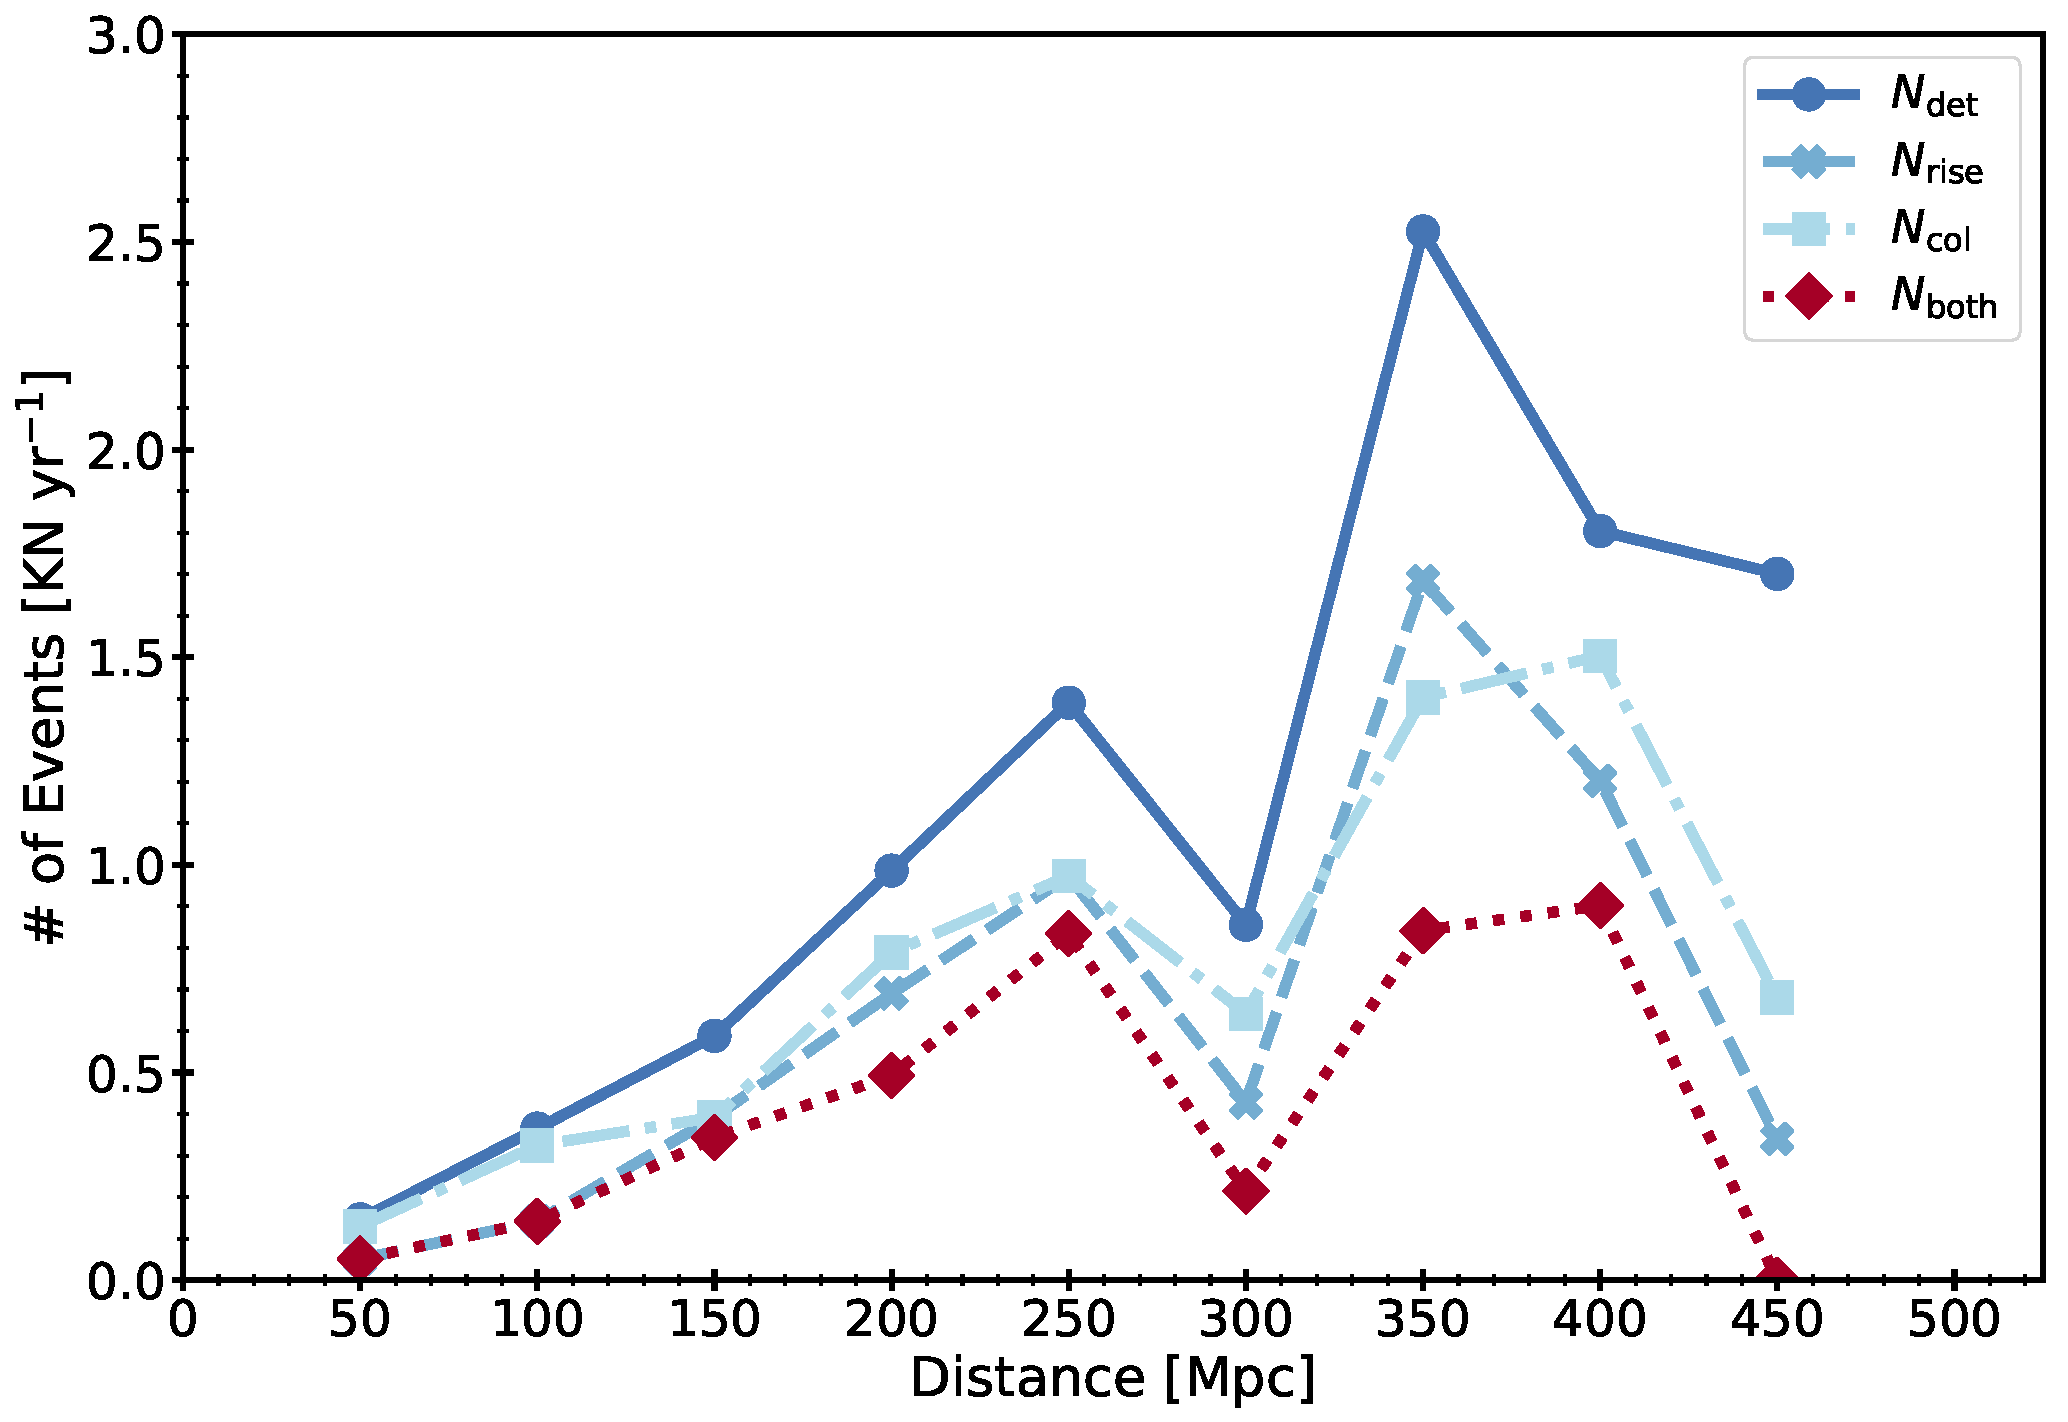
\includegraphics[width=0.95\textwidth]{./figs/chapter6/f1a.pdf}}
\caption{\singlespace Expected number of kilonova per year per distance bin, computed as described in \cref{sec:ch6_opsim_results}. The dip in expected numbers at 300~Mpc is simply the result of stochasticity in the simulation.}
\label{fig:ch6_eff_dist}
\end{center}
\end{figure}

\clearpage
Looking at \Cref{fig:ch6_eff_dist}, we first note that only the three brightest models (GW170817, {\tt h\_blue\_h\_red}, and {\tt h\_blue\_l\_red}) are detected. The model {\tt l\_blue\_h\_red}, is not detected despite having the same {\it total} ejecta mass as the model {\tt h\_blue\_l\_red}. This is because all the mass in the {\tt l\_blue\_h\_red} is contained in the high-opacity ``red" component and is therefore less luminous. The model {\tt l\_red\_l\_blue} is simply too faint to detect due to it's extremely low total ejecta mass. Inspecting \Cref{fig:ch6_eff_dist} for trends that depend on distance, we first note that there is a dip in the expected number at 300~Mpc. This feature can be attributed to stochasticity in the simulations. There is also a peak in the expected numbers around 350--400~Mpc. This represents the optimal position where there is a large volume probed, but sources are still nearby enough to be detected. Lastly, as expected, requiring stricter cuts on light curve behavior results in fewer detections.

The final point worth considering here is that this analysis has relied on an extremely minimal set of detection and characterization criteria. The light curves of kilonovae that satisfy these criteria will be sparsely sampled in both time and broadband filter coverage and we will not be able to make definitive statements about key properties such as color and timescale. As a result, it will in practice be difficult if not impossible to claim these as definitive kilonovae detections. Consequently, while a handful of kilonovae may appear in the LSST survey per year the overall science returns per event will be low.

\clearpage
\subsection{Benefits of Target of Opportunity Observations}
\label{sec:ch6_too_benefits}
The key point emerging from \cref{sec:ch6_opsim_results} is that despite the large \'{e}tendue of the LSST survey, it will be relatively inefficient at finding kilonova compared to other types of transient events. This low efficiency also suggests that the likelihood of a serendipitous joint detection between LIGO and LSST is vanishingly small. Even in the fortuitous situation of a joint detection, if it takes several days to detect and identify the kilonovae, this will severely limit our ability to perform multi-wavelength imaging and spectroscopy. These comprehensive multi-wavelength follow-up programs were found to be crucial for maximizing the science returns from GW170817.

The most obvious and effective way to combat this issue is by engaging in triggered target-of-opportunity observations. Consider such a campaign that invests no more than an hour or two per night for a few days to obtain deep images of the localization region with several broadband filters. These observations will be able to achieve depths that are 1.5--2 magnitudes deeper than the LSST main survey and consequently probe larger regions of the kilonovae ejecta parameter space (e.g., models such as {\tt l\_blue\_h\_red} and {\tt l\_red\_l\_blue}). These observations should commence promptly after the GW trigger is received to ensure that the crucial early-time light curve behavior is adequately captured. Furthermore, obtaining broadband imaging covering multiple filters allows accurate characterization of the rapidly evolving kilonova colors in a way that can not be achieved with sparse observations. Once a clear kilonova candidate (or handful of candidates) has been identified, further follow-up photometric and spectroscopic observations can be conducted using other telescopes allowing LSST to quickly return to main science operations.

\section{Discussion and Conclusion}
\label{sec:ch6_conc}
We have presented detailed simulated observations of kilonovae using LSST while considering two distinct contexts. First, we investigated the ability of LSST to both detect and characterize kilonovae over the course of the primary ten year survey. Second, we discuss the effectiveness of a triggered target-of-opportunity campaign conducted in response to a gravitational wave event trigger from the Advanced LIGO/Virgo interferometers. A key point that emerges from both considerations is that it may be difficult to detect kilonova in the main survey across the entire range of possible ejecta parameters. Models that have ejecta masses similar to or greater than those associated with GW170817 can be detected by LSST. However, models with lower ejecta mass quickly become too faint to observe effectively. We also show that the cadence of the LSST main survey is poorly matched to kilonovae timescales, leading to just a handful of detections per year. 

We instead argue that targeted ToO campaigns with a modest investment in telescope time (\apx~a~few~hours) can detect a wider range of kilonovae models across the entire Advanced LIGO/Virgo volume. The resulting kilonovae light curves from such a campaign will be far better sampled in both time and wavelength compared to those detected in the main survey, allowing detailed studies of the kilonovae behavior and properties. From this work, a clear picture emerges that LSST can and should play a vital and important role in the future of joint GW-EM astronomy. 